\documentclass[12pt, titlepage]{article}
\usepackage[utf8]{inputenc}
\usepackage{graphicx}
\usepackage{indentfirst}
\usepackage{array}
\usepackage{longtable}
\usepackage[a4paper,width=150mm,top=25mm,bottom=25mm]{geometry}

\title{Weather App Programmer Manual}

\author{Kyle Chestnut, Caleb Newman, Trey Coleman, Alan Huebschen}

\begin{document}

\maketitle

\section{Introduction}

\subsection{Scope}

Our group created a GUI based weather application which was written in Python and uses the PyQt bindings to create a user interface. When the program is first opened, it queries an external web server to get the user’s external IP. It then takes that IP and queries a location database service to find the approximate location of the IP. This location is then fed into the openweathermap public API which returns not only the current weather but also a 5 day forecast. Both current weather and the 5 day forecast are displayed on the user interface. The user can also search for a location and display the associated weather data with their requested location.

\subsection{Definitions}

No definitions, acronyms or abbreviations were used in the making of this document.

\subsection{Trademark and copyright statement}

No trademarked or copyrighted material was used to create this program.

\section{General Description}
\subsection{Product Perspective}

This software is being built for those people who just have no idea what the current weather is at their location. They happen to have an x64 windows 10 machine with an internet connection but can’t go outside. Perhaps they can go outside, but they also want to know what the near future weather will be like. Maybe they are worried about their mother who lives elsewhere and they want to check the weather out by her. This product will solve countless problems and save infinite lives.

\subsection{Product Functions}

This product will show the user’s current weather at their current location along with weather predicted for the next 5 days at noon. The user can also search for other locations’ weather and display the 5 day forecast for that location

\subsection{User Characteristics}

Person with windows 10 x64 machine and an internet connection who wants to know the current and future weather

\subsection{General Constraints}

MUST have internet access for API calls to work

\subsection{Assumptions and Dependencies}

MUST have an internet connection, windows 10 x64, and 300MB of storage

This project was built using Python 3.9, a Python 3.9 interpreter along with pip package manager is required for testing and building the executable.

\section{Specific Requirements}
\subsection{Tools}

\begin{itemize}
    \item VSCodium
    \item Python 3.9
    \item Pyinstaller
    \item Git
    \item Github
    \item PyQt5
    \item Qt Designer
\end{itemize}

\section{Known Bugs and Issues}
\subsection{Issues}
\begin{enumerate}
    \item When the user opens the program they may see data for a city that they are not located in.  This is because your internet service provider may be altering your IP in a way such that it matches a different city.  Location based on IP can also be inaccurate and it depends on the quality of the database being queried.
    \item When the user enters a city or a zip code it may not get the weather of the city the user is intending.  The best way to remedy this is to enter a zip code or an alternate zip code and thus will return an accurate result.
    \item When the user enters a city or a zip code it may not get the weather of the city the user is intending.  The best way to remedy this is to enter a zip code or an alternate zip code and thus will return an accurate result.
\end{enumerate}

\subsection{Bugs}

\begin{enumerate}
    \item When the user opens the program the query that gets their location may not recognize a city and thus will fail to launch the program.  
\end{enumerate}

\pagebreak
\section{Testing Documentation}

% \begin{tabular}{c|c|c|c|c}
%     Test Case # & Input & Expected Output & Rationale & Pass/Fail \\
%      & 
% \end{tabular}

% \usepackage{graphicx}


% \usepackage{array}


\begin{longtable}{>{\hspace{0pt}}m{0.048\linewidth}>{\hspace{0pt}}m{0.253\linewidth}>{\hspace{0pt}}m{0.196\linewidth}>{\hspace{0pt}}m{0.382\linewidth}>{\hspace{0pt}}m{0.044\linewidth}}
Test Case \# & Input & Expected Output & Rationale & Pass/ Fail \endfirsthead 
\hline
1 & Put in Very long text into prompt.~ Ex.~ Copy and paste hamlet & Catches the long output without crashing.~ Returns no town found. & We should limit the user to only input what is necessary for cities. & Pass \\
2 & Check for cursor blink throughout tests. & No output for this. & The user interface should not appear buggy. & Pass \\
3 & Drag and drop long text & Catches the long output without crashing.~ Returns no town found. & While copy and paste is allowed for longer city names.~ We should make sure that the input is valid. & Pass \\
4 & Check with different language options & Works normally, returning nothing if not recognized, or returning weather of location if accounted for by API & If users do not primarily use the english language we should account for whatever language they speak and write in. & Pass \\
5 & Hold down a single key for an extended period & Returns no town found. & We should only allow valid cities. & Pass \\
6 & Try to input an image in multiple fashions (different file types, drag and drop, copy and paste.) & Returns no town.~ Might just reject the input. & The text box should only allow for text input. & Pass \\
7 & Test for null/ blank & Does not search, or no town found. & Users may accidentally delete their city entry before getting their forecast & Pass \\
8 & Max character test & Catches that there are more characters than the box allows, or caps the amount of characters when put into the box. & There should not be a way for the user to “overflow” our program or the API we are using so a max length on the text box will be added & Pass \\
9 & Symbols of varying origin (Alt key symbols, characters from different alphabets, numbers, symbols, numbers, etc.) & Works normally, or returns default value. & Some cities may contain letters not a part of the English alphabet.~ As long as the city name is valid the city should be returned. & Pass \\
10 & Ascii characters. & Ascii is not supported and therefore should return an error. & The user should only be able to enter valid text. & Pass \\
11 & Control characters & Control characters are not supported and therefore should return an error & The user should only be able to enter valid text. & Pass \\
12 & Boundary values test & If the city is valid and is within the boundaries that have been set then we return the city.~ If not we return an error & The boundary values that were set for the text box should not be violated. & Pass \\
13 & Are the characters properly visible in text input? & Normal output.~ Should be able to see text input. & The user should clearly see what city they are attempting to input. & Pass \\
14 & Basic city name test & Returns the town name and weather~ & The user should be able to enter a town name and get the weather for that town. & Pass \\
15 & Basic zip code test & Returns the town name and weather based on the zip code provided. & The user should be able to enter a zip code and get the weather for that location. & Pass \\
16 & Check for pasting unusual characters in the text field. & Should not crash or glitch. & With unusual input the program itself should not crash and just return an error that a city cannot be found. & Pass \\
17 & Enter spaces in the prefix and suffix of what you type. & The program handles spaces before and after the town name, and return proper weather results & As long as the name of the town is valid, it should return the results. & Pass \\
18 & Does any elements of the program change position through repeated use of the program? & No output.~ Just watch. & The user should be able to input as many locations as they want in a singular run of the program.~ Although it will be done one at a time, the location of each component should be static and the information should not deviate from its original position. & Pass \\
19 & Check if repeatedly pressing the forecast button many times crashes the program or glitches it out.~ (do this with both an empty field and non empty field) & The program will function every time without crashing. & If the user is clicking the “Get Forecast” button repeatedly the program should function no differently. & Pass \\
20 & Check for only spaces as input. & Returns no city found because spaces are not a valid input for a city. & We want to account for most if not all cases of user input. & Pass \\
21 & Does copying from the text box work? & No crash or error. & A user should be able to copy and paste into the text box. & Pass \\
22 & Enter a mix of numbers and characters into the text box. & Return no city found & A user should be allowed to enter a city or zip code but not a combination of the two. & Pass \\
23 & Enter a city name with a space in the middle of the name. Example: Spring field & Return no city found & A user may accidentally space in the middle of a city name without noticing.~ We want to be able to catch that error & Pass \\
24 & Enter a city name with a space in the middle of a name.~\par{}Example: San Jose & Return the proper city and weather. & A user may enter a city that specifically has a space in between two words.~~ & Pass \\
25 & VPN and proxy & Should return the weather based on the default I.P. & Users may have an active VPN or proxy server on their machine. & Fail
\end{longtable}

\section{Design Documentation}
\subsection{Architecture Diagram}

\begin{center}
    \makebox[\textwidth]{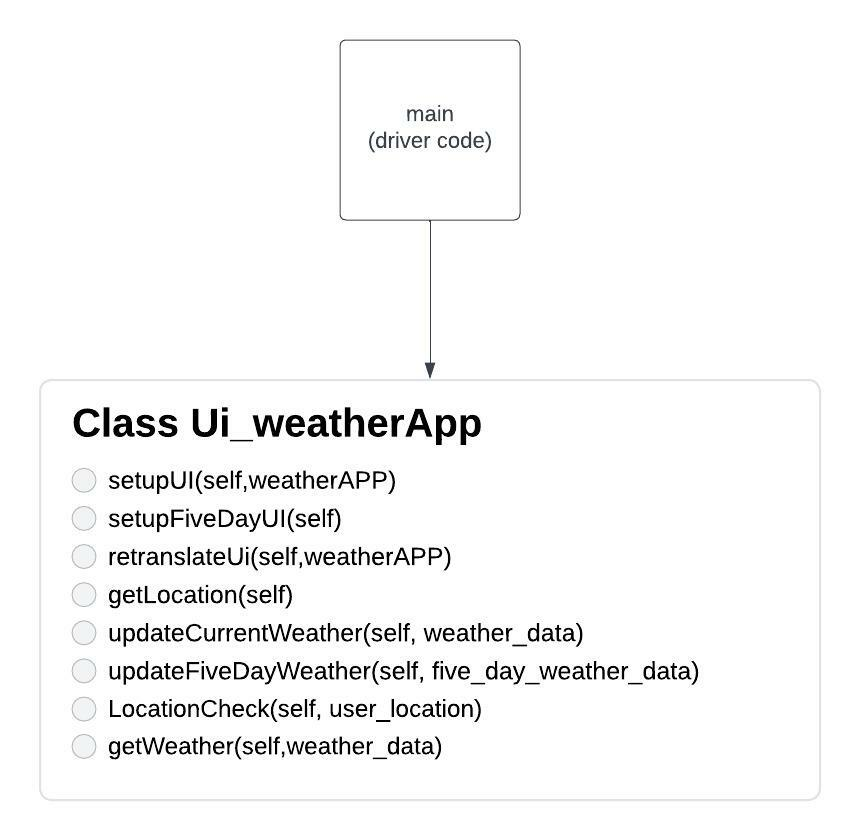
\includegraphics[width=\textwidth{...}]{architecture_diagram.png}}
\end{center}

\subsection{Flow Chart}
\begin{center}
    \makebox[\textwidth]{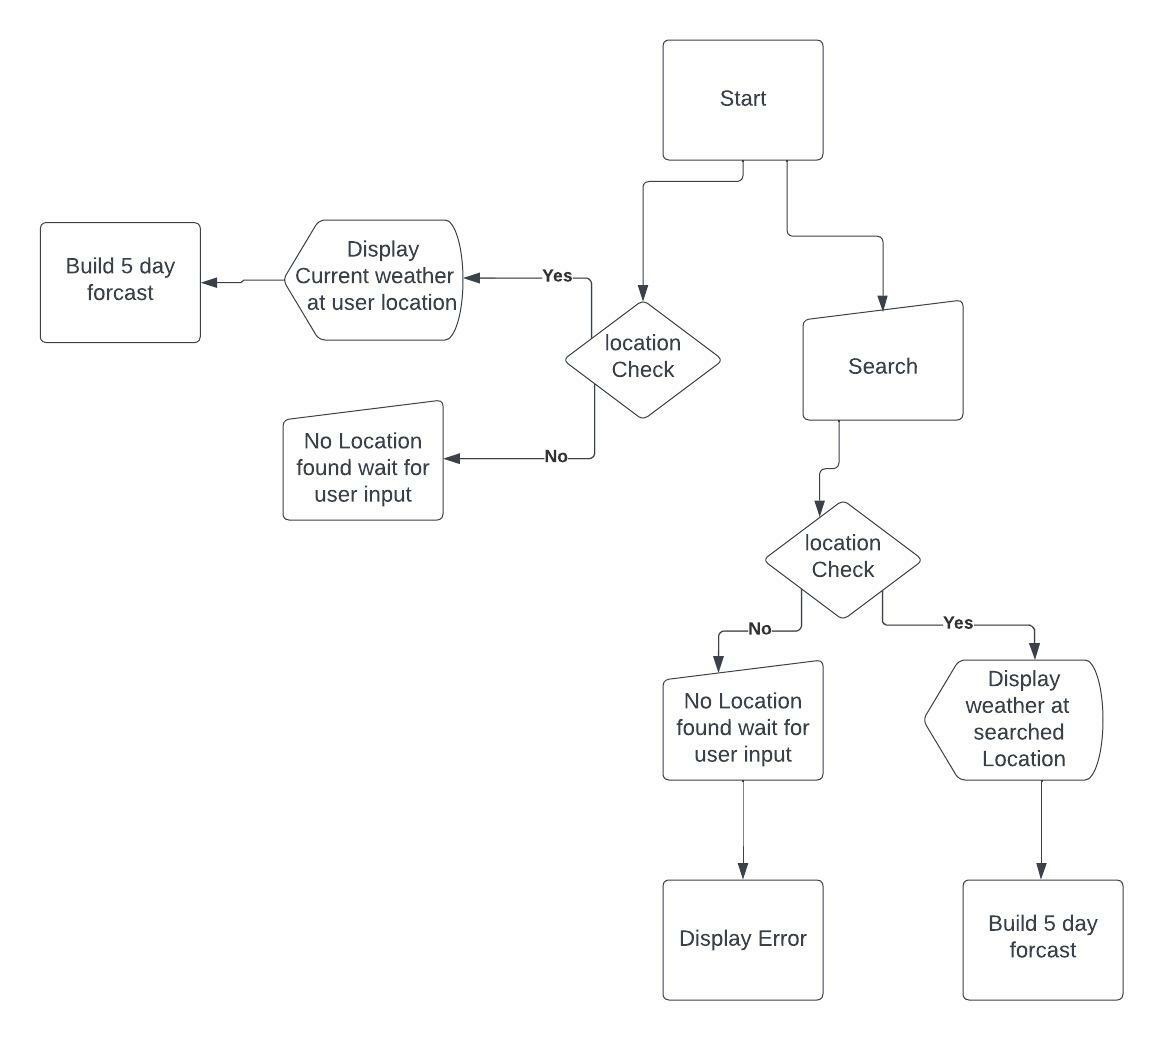
\includegraphics[width=\textwidth{...}]{flow_chart.jpg}}
\end{center}

\end{document}
